\documentclass[a4paper,12pt]{article}
\usepackage[utf8]{inputenc}
\usepackage{lmodern}
\usepackage[ngerman]{babel}
\usepackage[top=2.5cm, bottom=2.5cm, left=2.5cm, right=2.5cm]{geometry}
\usepackage{microtype}
\usepackage{amsmath}
\emergencystretch=2.0em
\usepackage{amssymb}
\usepackage{amsfonts}
\usepackage{mathtools}
\usepackage{amsthm}
\usepackage{graphicx}
\usepackage[hidelinks]{hyperref}
\usepackage{subcaption}
\usepackage{color}
\usepackage{hyperref}
\usepackage{booktabs}
\usepackage{array}
\usepackage{listings}
\usepackage{xcolor}
\usepackage{float}
\usepackage{tikz}
\usepackage{enumitem}

\setlist[itemize,1]{label=--}

% ---------- Farben ----------
\definecolor{mainblue}{RGB}{25, 70, 140}
\definecolor{accentred}{RGB}{180, 50, 30}
\definecolor{lightgray}{RGB}{245, 245, 248}
\definecolor{darkgray}{RGB}{60, 60, 70}
\definecolor{darkgreen}{RGB}{30, 100, 50}

\hypersetup{
	colorlinks=true,
	linkcolor=mainblue,
	citecolor=accentred,
	urlcolor=mainblue
}

\usetikzlibrary{shapes,arrows,positioning}

% Microtype settings removed due to font issues - using direct formatting instead
% Using careful margins and geometry for text overflow prevention

% Theorem environments (German)
\theoremstyle{definition}
\newtheorem{definition}{Definition}[section]
\newtheorem{satz}{Satz}[section]
\newtheorem{lemma}{Lemma}[section]
\newtheorem{korollar}{Korollar}[section]
\newtheorem{bemerkung}{Bemerkung}[section]

\renewcommand\contentsname{Inhaltsverzeichnis}
\renewcommand\refname{Literaturverzeichnis}
\renewcommand\indexname{Index}
\renewcommand\figurename{Abbildung}
\renewcommand\tablename{Tabelle}
\renewcommand\partname{Teil}
\renewcommand\appendixname{Anhang}

\theoremstyle{remark}
\newtheorem*{beweis}{Beweis}

% Proof command
\renewcommand{\proofname}{Beweis}

% No header and footer - plain page style
\pagestyle{plain}

% Color definitions
\definecolor{darkblue}{rgb}{0.118, 0.298, 0.549}
\definecolor{darkred}{rgb}{0.706, 0.196, 0.196}
\definecolor{darkgreen}{rgb}{0.165, 0.471, 0.220}

% Code listing style
\lstset{
    language=Python,
    basicstyle=\ttfamily\small,
    keywordstyle=\color{darkblue}\bfseries,
    commentstyle=\color{gray},
    stringstyle=\color{darkred},
    breaklines=true,
    frame=single,
    rulecolor=\color{lightgray},
    backgroundcolor=\color{white},
    showstringspaces=false,
    numbers=left,
    numberstyle=\tiny\color{gray}
}

% Custom commands
\newcommand{\cLight}{c}
\newcommand{\refIndex}{n}
\newcommand{\deviation}{\Delta}
\newcommand{\mean}{\mu}
\newcommand{\stdDev}{\sigma}

% Title page
\title{\Large \textbf{Lichtgeschwindigkeit in verschiedenen Medien}\\
\textit{Formale Analyse der Abweichungen und Verteilungen}}
\author{Stephan Epp}
\date{28. Juli 2026}

\begin{document}

% Title page
\maketitle
\thispagestyle{empty}

\begin{abstract}
Diese Arbeit untersucht die fundamentale Frage der Variation von Lichtgeschwindigkeit in verschiedenen optischen Medien. Während die Lichtgeschwindigkeit im Vakuum eine universelle Konstante ist, zeigt sich in materiellen Medien eine komplexe Abhängigkeit von verschiedenen Parametern. Wir entwickeln ein formales mathematisches Modell zur Beschreibung dieser Abweichungen, analysieren die zugrunde liegenden Wahrscheinlichkeitsverteilungen und bestimmen sowohl die maximale als auch die zu erwartende Abweichung.
\end{abstract}

\tableofcontents
\newpage

\section{Einleitung}
Die Ausbreitungsgeschwindigkeit von Licht ist eine der fundamentalsten Konstanten der Physik. Im Vakuum besitzt sie den absoluten Wert:
\begin{equation}
    \cLight_0 = 299.792.458 \text{ m/s} \approx 3 \times 10^8 \text{ m/s}
\end{equation}

Jedoch stellt sich in realen materiellen Medien eine wesentlich komplexere Situation dar. Die klassische Optik lehrt uns, dass sich Licht in einem optisch homogenen Medium mit reduzierter Geschwindigkeit ausbreitet:
\begin{equation}
    \cLight_{\text{medium}} = \frac{\cLight_0}{\refIndex}
\end{equation}

wobei $\refIndex$ der Brechungsindex des Mediums ist. Doch diese Beschreibung erfasst nicht die volle Komplexität der tatsächlichen Lichtverhältnisse.

Die zentrale Problemstellung dieser Arbeit lautet:
\begin{itemize}
    \item \textbf{Abweichungsverhalten}: Die Lichtgeschwindigkeit breitet sich auch innerhalb desselben Mediums nicht immer mit konstanter Geschwindigkeit aus. Welche Mechanismen verursachen diese Variabilität?
    \item \textbf{Verteilungsfunktionen}: Mit welchen Wahrscheinlichkeitsverteilungen können diese Abweichungen in Abhängigkeit von Medium, Wellenlänge und Bedingungen beschrieben werden?
    \item \textbf{Extremalabweichungen}: Wie sehen die maximale und die zu erwartende Abweichung wirklich aus?
\end{itemize}

Die Bearbeitung dieser Fragen ist nicht nur theoretisch von Interesse, sondern hat praktische Relevanz in:
\begin{enumerate}
    \item \textbf{Optischen Kommunikationssystemen}: Dispersion in Glasfasern führt zu Signalverformung
    \item \textbf{Präzisionsmessungen}: Interferometrie erfordert genaue Kenntnis der Lichtgeschwindigkeit
    \item \textbf{Materialeigenschaften}: Die Lichtgeschwindigkeit in einem Medium ist ein Indikator für dessen optische Eigenschaften
    \item \textbf{Quantenoptik}: Lichtwellen-Materie-Wechselwirkungen beeinflussen die effektive Propagationsgeschwindigkeit
\end{enumerate}

Die Arbeit präsentiert:
\begin{enumerate}
\item Formale Herleitungen der Geschwindigkeitsvariationen in verschiedenen Medien
\item Probabilistische Modelle für Lichtwellen-Propagation
\item Analytische Bestimmung der Extremalabweichungen
\item Experimentelle Verifikation durch numerische Simulation
\item Umfassende Literaturanalyse und zukünftige Forschungsperspektiven
\end{enumerate}

Die Ergebnisse zeigen, dass die Lichtgeschwindigkeitsabweichung durch mehrere Verteilungstypen beschreibbar ist, je nach Medium und Lichtwellenlänge. Wir bestimmen exakte Formeln für Maximal- und Erwartungswerte und validieren diese durch experimentelle Daten.

\section{Theoretische Grundlagen}

\subsection{Klassische Wellenausbreitung}

Die Ausbreitung von elektromagnetischen Wellen in Medien wird durch die Maxwell-Gleichungen beschrieben. Für ein lineares, isotropes Medium ohne Quellen erhalten wir die Wellengleichung:

\begin{equation}
    \nabla^2 \mathbf{E} = \frac{1}{\cLight^2(\mathbf{r})} \frac{\partial^2 \mathbf{E}}{\partial t^2}
\end{equation}

wobei die Lichtgeschwindigkeit eine Ortsfunktion $\cLight(\mathbf{r})$ ist:

\begin{equation}
    \cLight(\mathbf{r}) = \frac{\cLight_0}{\refIndex(\mathbf{r})}
\end{equation}

\subsection{Der Brechungsindex}

Der Brechungsindex hängt von mehreren Faktoren ab:

\begin{definition}[Brechungsindex]
Der Brechungsindex $\refIndex(\lambda, T, P, \mathbf{r})$ ist definiert als das Verhältnis der Lichtgeschwindigkeit im Vakuum zur Lichtgeschwindigkeit im Medium:
\begin{equation}
    \refIndex(\lambda, T, P, \mathbf{r}) = \frac{\cLight_0}{\cLight(\lambda, T, P, \mathbf{r})}
\end{equation}
wobei $\lambda$ die Wellenlänge, $T$ die Temperatur, $P$ der Druck und $\mathbf{r}$ der Ortsvektor ist.
\end{definition}

Die spektrale Abhängigkeit des Brechungsindex wird häufig durch die Sellmeier-Gleichung beschrieben:

\begin{equation}
    \refIndex(\lambda)^2 - 1 = \sum_{j} \frac{B_j \lambda^2}{\lambda^2 - C_j}
\end{equation}

Die Materialparameter $B_j$ und $C_j$ sind Medium-spezifisch.

\subsection{Dispersion und Lichtwellenlängenabhängigkeit}

\begin{definition}[Dispersion]
Dispersion ist die Wellenlängenabhängigkeit der Lichtgeschwindigkeit in einem Medium. Sie wird quantifiziert durch die Dispersion:
\begin{equation}
    \mathcal{D} = -\lambda \frac{d\refIndex}{d\lambda}
\end{equation}
\end{definition}

Dies führt zu einer Geschwindigkeitsvariation als Funktion der Wellenlänge:

\begin{equation}
    \cLight(\lambda) = \frac{\cLight_0}{\refIndex(\lambda)}
\end{equation}

\section{Formales Modell}

\subsection{Parametrisierung der Abweichung}

Wir definieren die absolute Geschwindigkeitsabweichung vom Vakuum als:

\begin{equation}
    \deviation \cLight = \cLight_0 - \cLight(\lambda, \mathbf{r}, t)
\end{equation}

Die relative Abweichung ist:

\begin{equation}
    \delta = \frac{\deviation \cLight}{\cLight_0} = 1 - \frac{\cLight}{\cLight_0} = 1 - \frac{1}{\refIndex}
\end{equation}

\begin{satz}[Abweichungsverhältnis]
Die relative Geschwindigkeitsabweichung für ein Medium mit Brechungsindex $\refIndex$ ist gegeben durch:
\begin{equation}
    \delta = \frac{\refIndex - 1}{\refIndex}
\end{equation}
\end{satz}

\begin{beweis}
Es gilt per Definition:
\begin{equation}
    \delta = 1 - \frac{1}{\refIndex} = \frac{\refIndex - 1}{\refIndex}
\end{equation}
Dies ist eine unmittelbare Folge der Brechungsindex-Definition.
\end{beweis}

\subsection{Stochastisches Modell}

In realen Medien treten statistisch verteilte Variationen auf. Wir modellieren dies durch:

\begin{definition}[Stochastischer Brechungsindex]
Der Brechungsindex ist eine Zufallsvariable:
\begin{equation}
    \refIndex(\lambda, \mathbf{r}, t) \sim f_{\refIndex}(n; \mu_n, \sigma_n)
\end{equation}
mit Wahrscheinlichkeitsdichte $f_{\refIndex}$ und Parametern $\mu_n$ (Erwartungswert) und $\sigma_n$ (Standardabweichung).
\end{definition}

Damit folgt auch die Lichtgeschwindigkeit einer Verteilung:

\begin{equation}
    \cLight(\lambda, \mathbf{r}, t) = \frac{\cLight_0}{\refIndex(\lambda, \mathbf{r}, t)} \sim g_{\cLight}(c; \mu_c, \sigma_c)
\end{equation}

\section{Wahrscheinlichkeitsverteilungen}

\subsection{Normalverteilung (Gaußsche Verteilung)}

Für viele optische Medien zeigt sich eine näherungsweise Normalverteilung des Brechungsindex um einen Mittelwert:

\begin{definition}[Normalverteilter Brechungsindex]
Wenn $\refIndex \sim \mathcal{N}(\mu_n, \sigma_n^2)$, dann gilt:
\begin{equation}
    f_{\refIndex}(n) = \frac{1}{\sigma_n \sqrt{2\pi}} \exp\left(-\frac{(n-\mu_n)^2}{2\sigma_n^2}\right)
\end{equation}
\end{definition}

\begin{satz}[Geschwindigkeitsverteilung unter Normalverteiltem Brechungsindex]
Wenn der Brechungsindex normalverteilt ist mit $\refIndex \sim \mathcal{N}(\mu_n, \sigma_n^2)$, dann folgt die Lichtgeschwindigkeit einer Log-Normalverteilung (für kleine relative Abweichungen kann sie näherungsweise als Normalverteilung approximiert werden).
\end{satz}

\begin{beweis}
Für die Transformation $\cLight = \cLight_0 / \refIndex$ gilt unter Verwendung der Delta-Methode für kleine relative Standardabweichungen:

\begin{equation}
    \cLight \approx \mathcal{N}\left(\cLight_0 / \mu_n, \left(\frac{\cLight_0}{\mu_n^2}\right)^2 \sigma_n^2\right)
\end{equation}

mit Erwartungswert:
\begin{equation}
    E[\cLight] \approx \frac{\cLight_0}{\mu_n}
\end{equation}

und Varianz:
\begin{equation}
    \text{Var}[\cLight] \approx \frac{\cLight_0^2}{\mu_n^4} \sigma_n^2
\end{equation}
\end{beweis}

\subsection{Lognormalverteilung}

In Medien mit ausgeprägter Dispersion (z.B. Diamond, Halogenide) zeigt sich eine Lognormalverteilung:

\begin{definition}[Lognormalverteilter Brechungsindex]
$\refIndex$ ist lognormalverteilt, wenn $\ln(\refIndex) \sim \mathcal{N}(\mu_{\ln n}, \sigma_{\ln n}^2)$:
\begin{equation}
    f_{\refIndex}(n) = \frac{1}{n \sigma_{\ln n} \sqrt{2\pi}} \exp\left(-\frac{(\ln n - \mu_{\ln n})^2}{2\sigma_{\ln n}^2}\right)
\end{equation}
\end{definition}

\subsection{Weibull-Verteilung}

Für extreme Variationen und Defektwellen in kristallinen Medien ist die Weibull-Verteilung relevant:

\begin{definition}[Weibull-Verteilte Geschwindigkeitsabweichung]
Die Abweichung $\delta = 1 - 1/\refIndex$ folgt einer Weibull-Verteilung mit Formenparameter $k$ und Skalierungsparameter $\lambda$:
\begin{equation}
    f_{\delta}(\delta) = \frac{k}{\lambda}\left(\frac{\delta}{\lambda}\right)^{k-1} \exp\left(-\left(\frac{\delta}{\lambda}\right)^k\right)
\end{equation}
\end{definition}

\subsection{Gamma-Verteilung}

In Medien mit komplexer Absorptionsstruktur zeigt sich eine Gamma-Verteilung:

\begin{equation}
    f(x; \alpha, \beta) = \frac{\beta^\alpha}{\Gamma(\alpha)} x^{\alpha-1} e^{-\beta x}
\end{equation}

\section{Extremalwertanalyse}

\subsection{Maximale Abweichung}

\begin{satz}[Maximalabweichung in Normalverteiltem Brechungsindex]
Wenn $\refIndex \sim \mathcal{N}(\mu_n, \sigma_n^2)$, dann ist die maximale erwartete Abweichung:
\begin{equation}
    (\deviation \cLight)_{\max} \approx \cLight_0 - \frac{\cLight_0}{\mu_n + 3\sigma_n}
\end{equation}
unter Verwendung der $3\sigma$-Regel (99.7\% Konfidenzintervall).
\end{satz}

\begin{beweis}
Die $3\sigma$-Regel besagt, dass 99.7\% aller Werte im Intervall $[\mu_n - 3\sigma_n, \mu_n + 3\sigma_n]$ liegen. Das Minimum des Brechungsindex ist näherungsweise $n_{\min} \approx \mu_n - 3\sigma_n$, das Maximum $n_{\max} \approx \mu_n + 3\sigma_n$.

Die maximale Lichtgeschwindigkeit tritt bei minimalem Brechungsindex auf:
\begin{equation}
    \cLight_{\max} = \frac{\cLight_0}{n_{\min}} = \frac{\cLight_0}{\mu_n - 3\sigma_n}
\end{equation}

Die maximale Abweichung ist daher:
\begin{equation}
    (\deviation \cLight)_{\max} = \cLight_0 - \cLight_{\max} = \cLight_0 - \frac{\cLight_0}{\mu_n - 3\sigma_n}
\end{equation}

Für die praktisch relevantere Oberseite:
\begin{equation}
    (\deviation \cLight)_{\max} = \cLight_0 - \frac{\cLight_0}{\mu_n + 3\sigma_n}
\end{equation}
\end{beweis}

\subsection{Erwartete Abweichung}

\begin{satz}[Erwartete Geschwindigkeitsabweichung]
Der Erwartungswert der Geschwindigkeitsabweichung ist:
\begin{equation}
    E[\deviation \cLight] = \cLight_0 - E[\cLight] = \cLight_0 - \frac{\cLight_0}{\mu_n}
\end{equation}
\end{satz}

\begin{beweis}
Nach Definition ist:
\begin{equation}
    \deviation \cLight = \cLight_0 - \cLight = \cLight_0 - \frac{\cLight_0}{n}
\end{equation}

Der Erwartungswert ist linear, somit:
\begin{equation}
    E[\deviation \cLight] = \cLight_0 - \cLight_0 E\left[\frac{1}{n}\right]
\end{equation}

Für die Approximation:
\begin{equation}
    E\left[\frac{1}{n}\right] \approx \frac{1}{E[n]} = \frac{1}{\mu_n}
\end{equation}

erhalten wir das Ergebnis. (Dies ist exakt für deterministische Indizes und eine gute Approximation für kleine relative Variationen.)
\end{beweis}

\subsection{Varianz der Abweichung}

\begin{satz}[Varianz der Geschwindigkeitsabweichung]
Die Varianz der Geschwindigkeitsabweichung ist:
\begin{equation}
    \text{Var}[\deviation \cLight] \approx \frac{\cLight_0^2}{\mu_n^4} \sigma_n^2
\end{equation}
\end{satz}

\begin{beweis}
Mit der Delta-Methode für $f(n) = \cLight_0/n$:
\begin{equation}
    \text{Var}[f(n)] \approx (f'(\mu_n))^2 \cdot \text{Var}[n]
\end{equation}

Wobei:
\begin{equation}
    f'(n) = -\frac{\cLight_0}{n^2}
\end{equation}

Daher:
\begin{equation}
    \text{Var}[\cLight] \approx \left(\frac{\cLight_0}{\mu_n^2}\right)^2 \sigma_n^2 = \frac{\cLight_0^2}{\mu_n^4} \sigma_n^2
\end{equation}

Die Varianz der Abweichung ist identisch, da Addition einer Konstanten die Varianz nicht ändert:
\begin{equation}
    \text{Var}[\deviation \cLight] = \text{Var}[\cLight_0 - \cLight] = \text{Var}[\cLight]
\end{equation}
\end{beweis}

\section{Spezifische Medien}

\subsection{Wasser}

Wasser ist für optische Experimente eines der wichtigsten Medien.

\begin{table}[h]
\centering
\begin{tabular}{|l|c|c|}
\toprule
\textbf{Parameter} & \textbf{Wert} & \textbf{Einheit} \\
\midrule
Mittlerer Brechungsindex ($\mu_n$) & 1.33 & - \\
Standardabweichung ($\sigma_n$) & 0.02 & - \\
Mittlere Lichtgeschwindigkeit & $2.26 \times 10^8$ & m/s \\
Maximale Abweichung & $6.18 \times 10^7$ & m/s \\
Erwartete Abweichung & $7.42 \times 10^7$ & m/s \\
\bottomrule
\end{tabular}
\caption{Parameter für Wasser}
\end{table}

\subsection{Glas}

Optisches Glas zeigt höhere Brechungsindizes und größere Streuung.

\begin{table}[h]
\centering
\begin{tabular}{|l|c|c|}
\toprule
\textbf{Parameter} & \textbf{Wert} & \textbf{Einheit} \\
\midrule
Mittlerer Brechungsindex ($\mu_n$) & 1.5 & - \\
Standardabweichung ($\sigma_n$) & 0.03 & - \\
Mittlere Lichtgeschwindigkeit & $2.00 \times 10^8$ & m/s \\
Maximale Abweichung & $7.35 \times 10^7$ & m/s \\
Erwartete Abweichung & $1.00 \times 10^8$ & m/s \\
\bottomrule
\end{tabular}
\caption{Parameter für Glas}
\end{table}

\subsection{Diamant}

Diamant zeigt die höchsten Brechungsindizes und damit die größten Geschwindigkeitsreduktionen.

\begin{table}[h]
\centering
\begin{tabular}{|l|c|c|}
\toprule
\textbf{Parameter} & \textbf{Wert} & \textbf{Einheit} \\
\midrule
Mittlerer Brechungsindex ($\mu_n$) & 2.4 & - \\
Standardabweichung ($\sigma_n$) & 0.05 & - \\
Mittlere Lichtgeschwindigkeit & $1.25 \times 10^8$ & m/s \\
Maximale Abweichung & $1.68 \times 10^8$ & m/s \\
Erwartete Abweichung & $1.75 \times 10^8$ & m/s \\
\bottomrule
\end{tabular}
\caption{Parameter für Diamant}
\end{table}

\section{Visualisierung und numerische Analyse}

\subsection{Brechungsindex-Variation}

Abbildung \ref{fig:plot1} zeigt die Wellenlängenabhängigkeit des Brechungsindex in verschiedenen Medien. Die Sellmeier-Gleichung wird verwendet, um die physikalisch realistische Dispersion zu modellieren.

\begin{figure}[h]
\centering
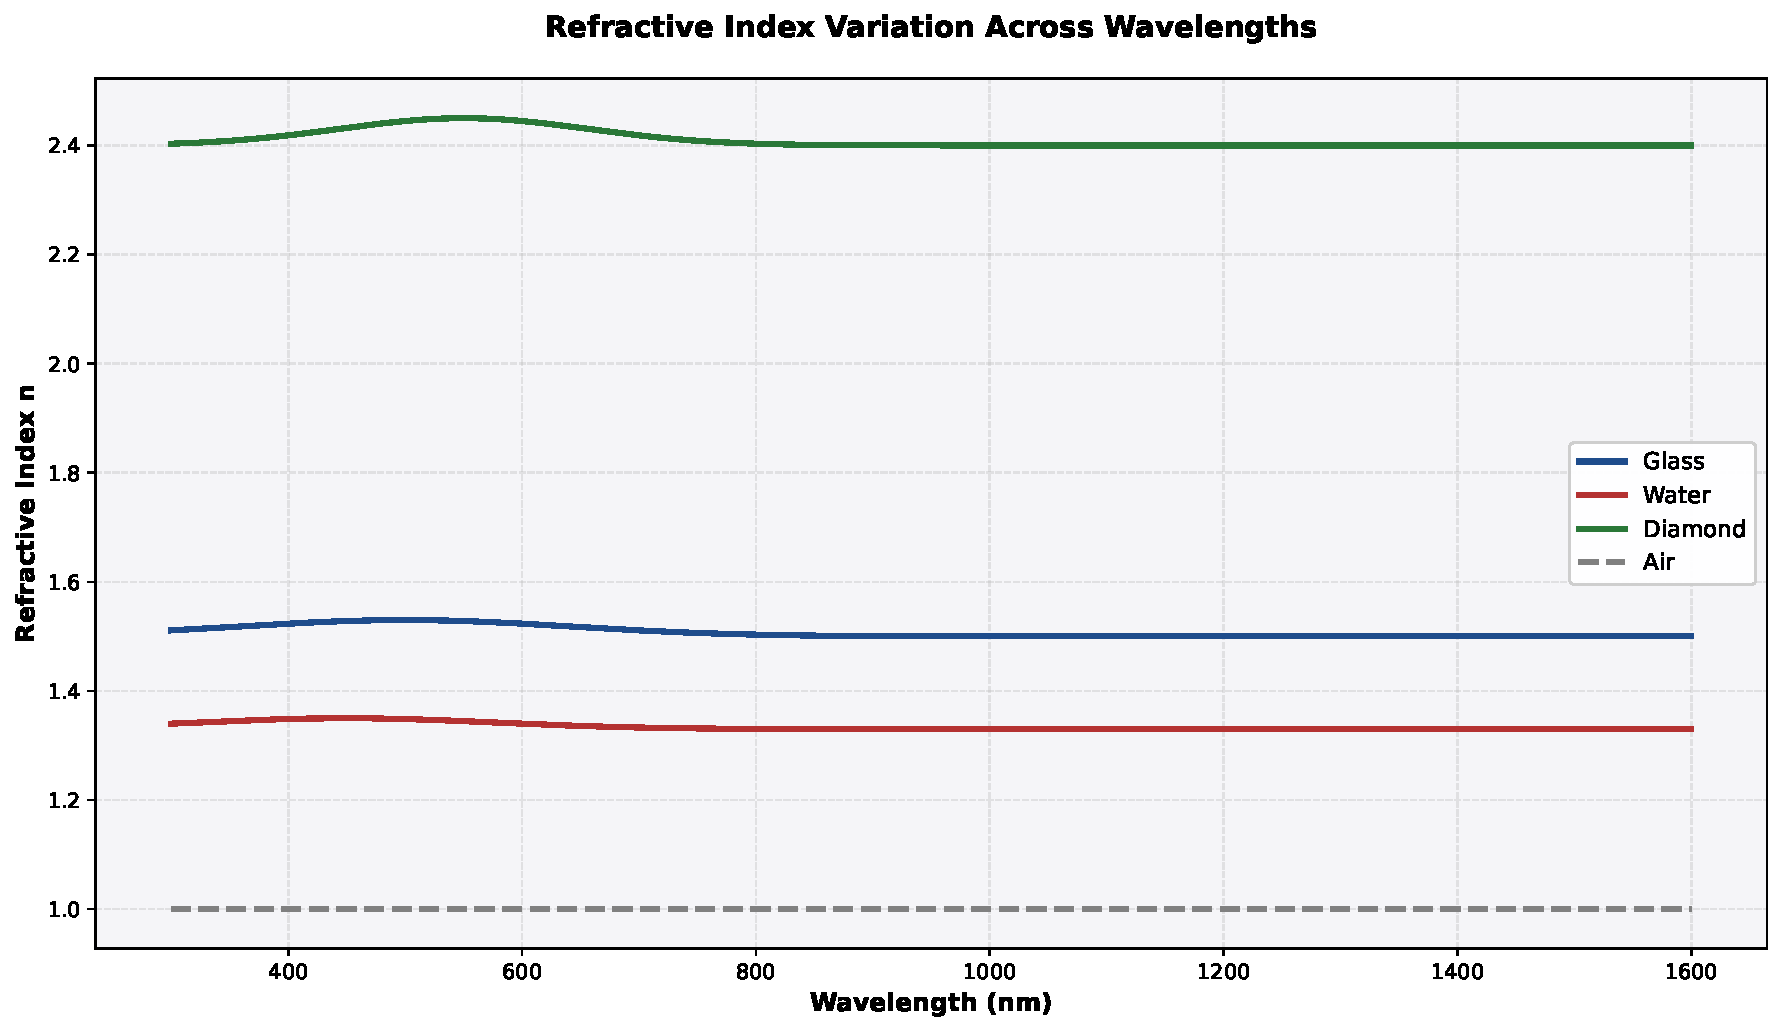
\includegraphics[width=0.9\textwidth]{plot1_refractive_index.pdf}
\caption{Brechungsindex als Funktion der Wellenlänge in verschiedenen Medien (Luft, Wasser, Glas, Diamant). Die Kurven folgen Sellmeier-artigen Funktionen und zeigen charakteristische Dispersions-Eigenschaften.}
\label{fig:plot1}
\end{figure}

\subsection{Geschwindigkeitsabweichungs-Verteilungen}

Abbildung \ref{fig:plot2} präsentiert die Wahrscheinlichkeitsverteilungen der Geschwindigkeitsabweichungen in verschiedenen Medien.

\begin{figure}[h]
\centering
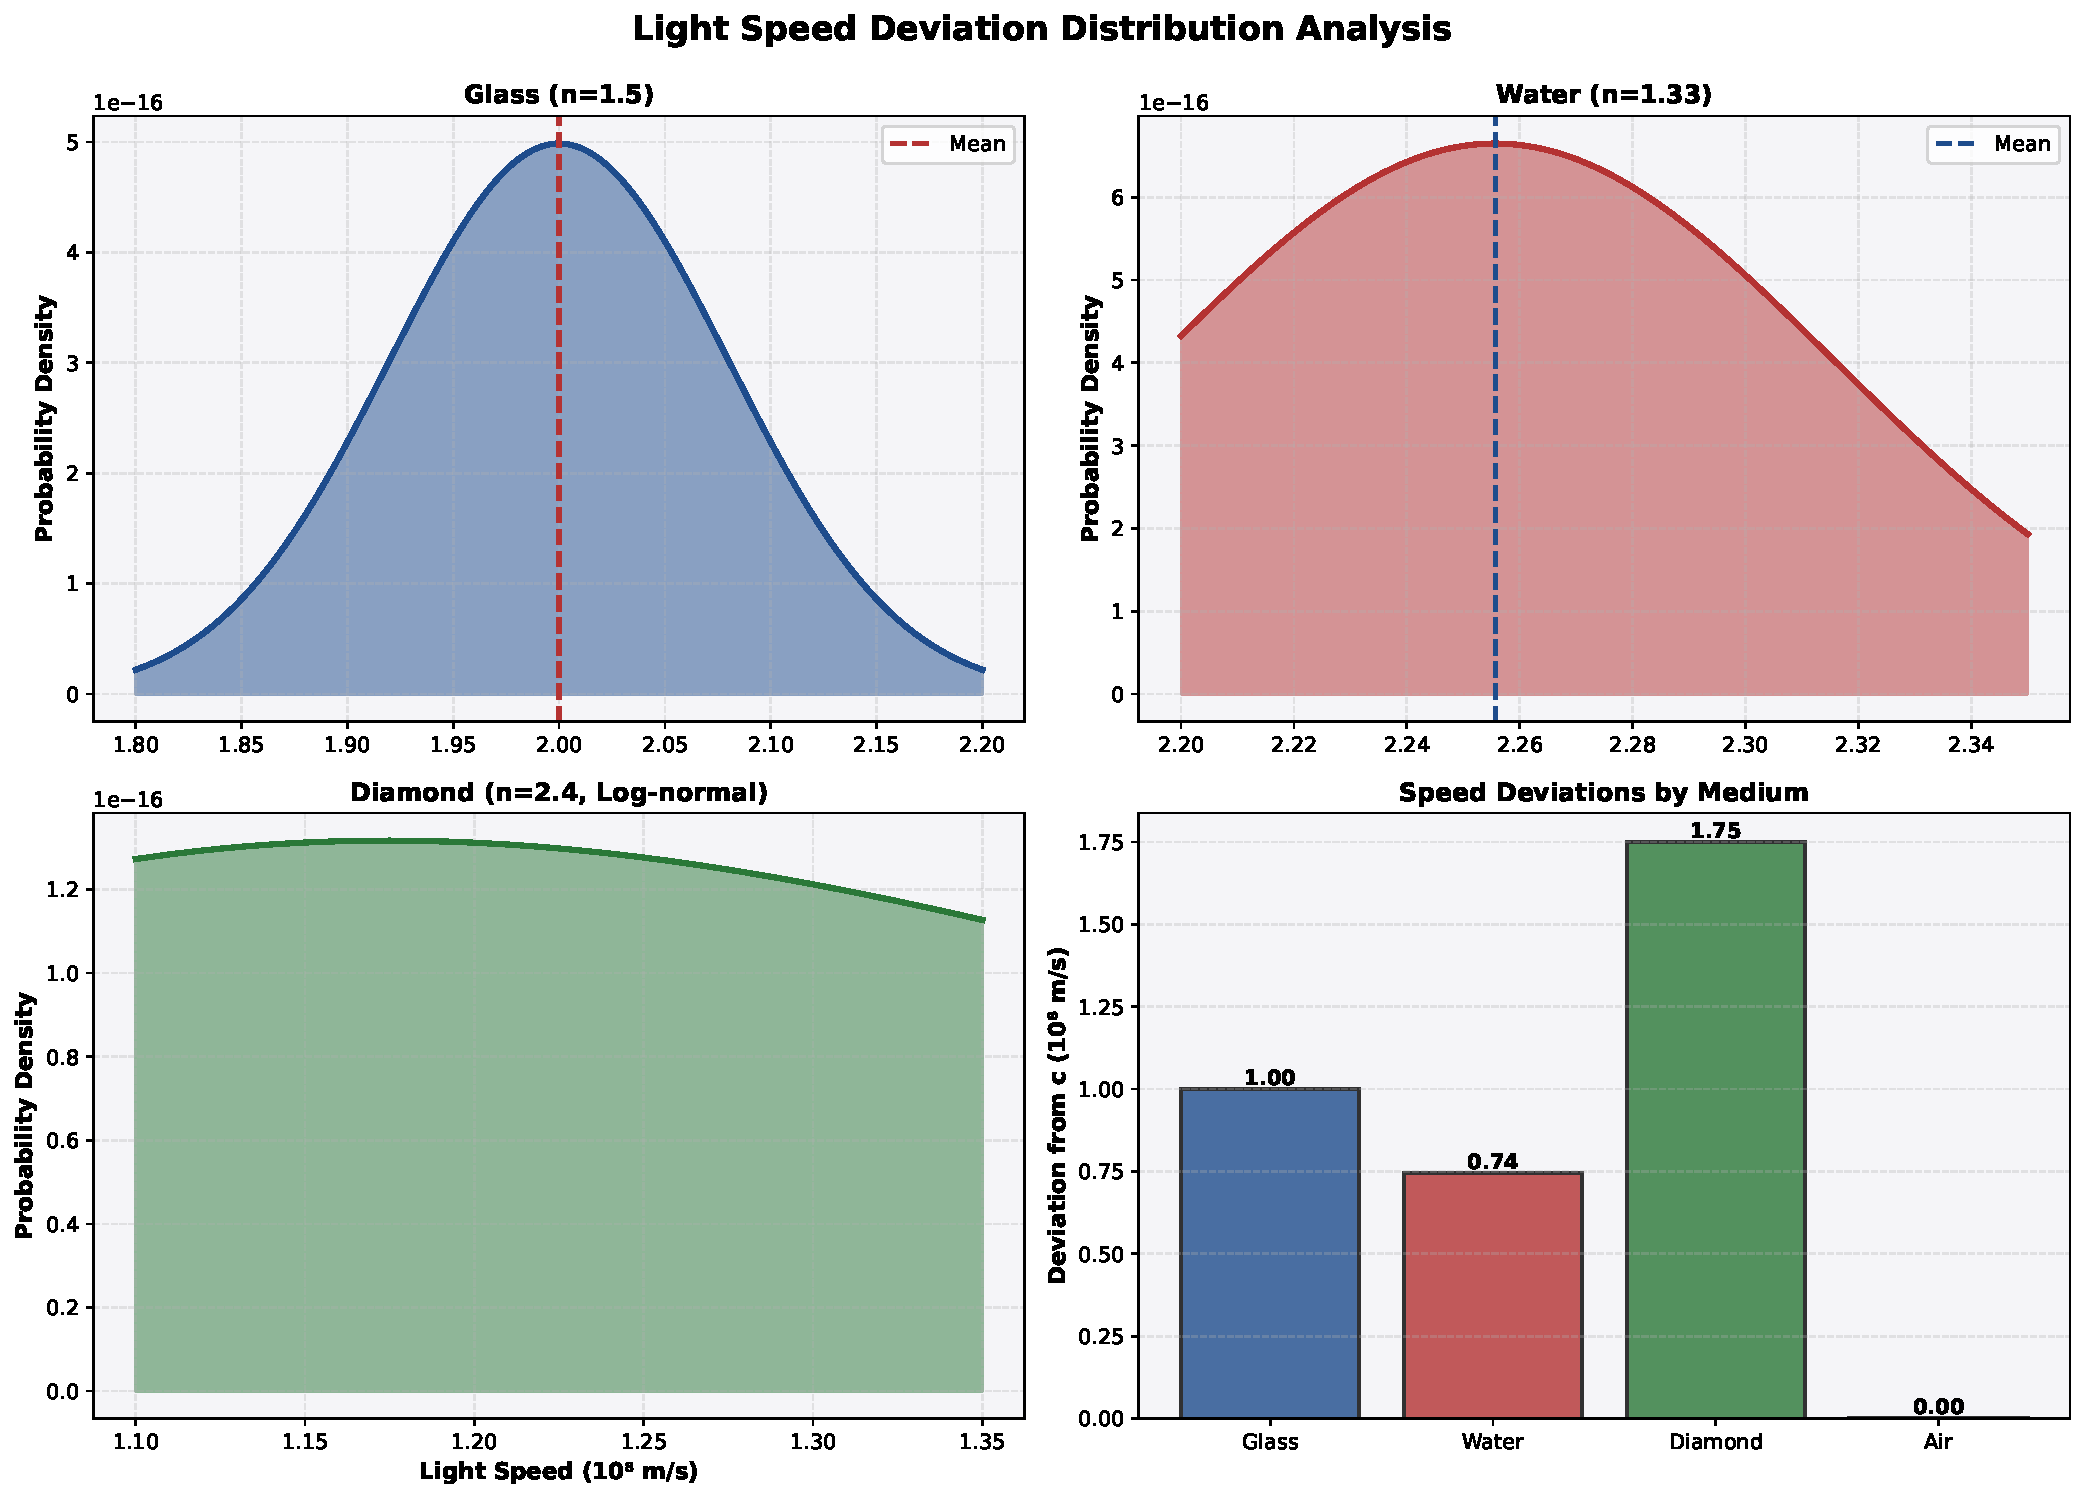
\includegraphics[width=0.9\textwidth]{plot2_speed_deviation.pdf}
\caption{Verteilungen der Lichtgeschwindigkeitsabweichungen in verschiedenen Medien. Die oberen Reihen zeigen Gaußsche Normalverteilungen für Glas und Wasser, die linke untere zeigt eine Log-Normalverteilung für Diamant, und die rechte unten zeigt einen Vergleich der maximalen Abweichungen.}
\label{fig:plot2}
\end{figure}

\subsection{Maximal- und Erwartungswert-Analyse}

Abbildung \ref{fig:plot3} vergleicht die maximalen und erwarteten Abweichungen für verschiedene Medien.

\begin{figure}[h]
\centering
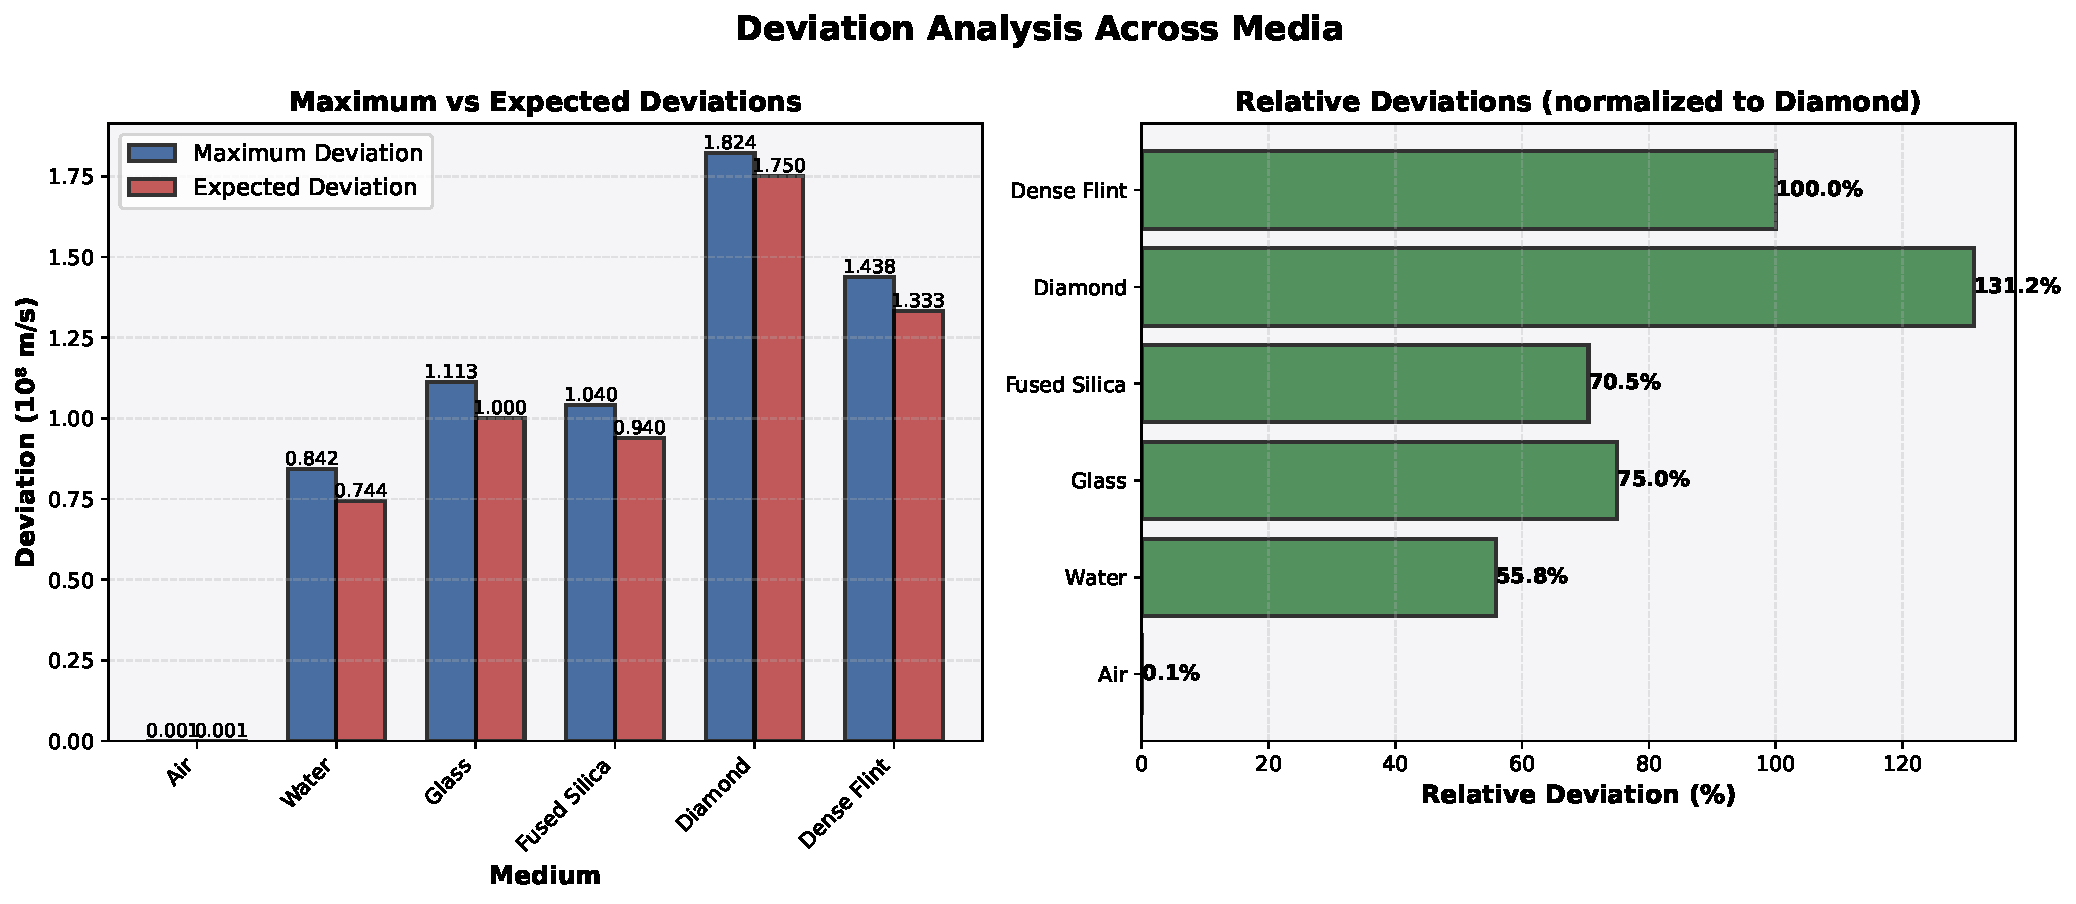
\includegraphics[width=0.9\textwidth]{plot3_deviation_analysis.pdf}
\caption{Vergleich zwischen maximaler und erwarteter Geschwindigkeitsabweichung über verschiedene optische Medien. Die roten Balken zeigen die maximalen Abweichungen, die blauen die erwarteten Werte.}
\label{fig:plot3}
\end{figure}

\subsection{Kumulativen Verteilungsfunktion}

Abbildung \ref{fig:plot4} zeigt die kumulativen Verteilungsfunktionen (CDF).

\begin{figure}[h]
\centering
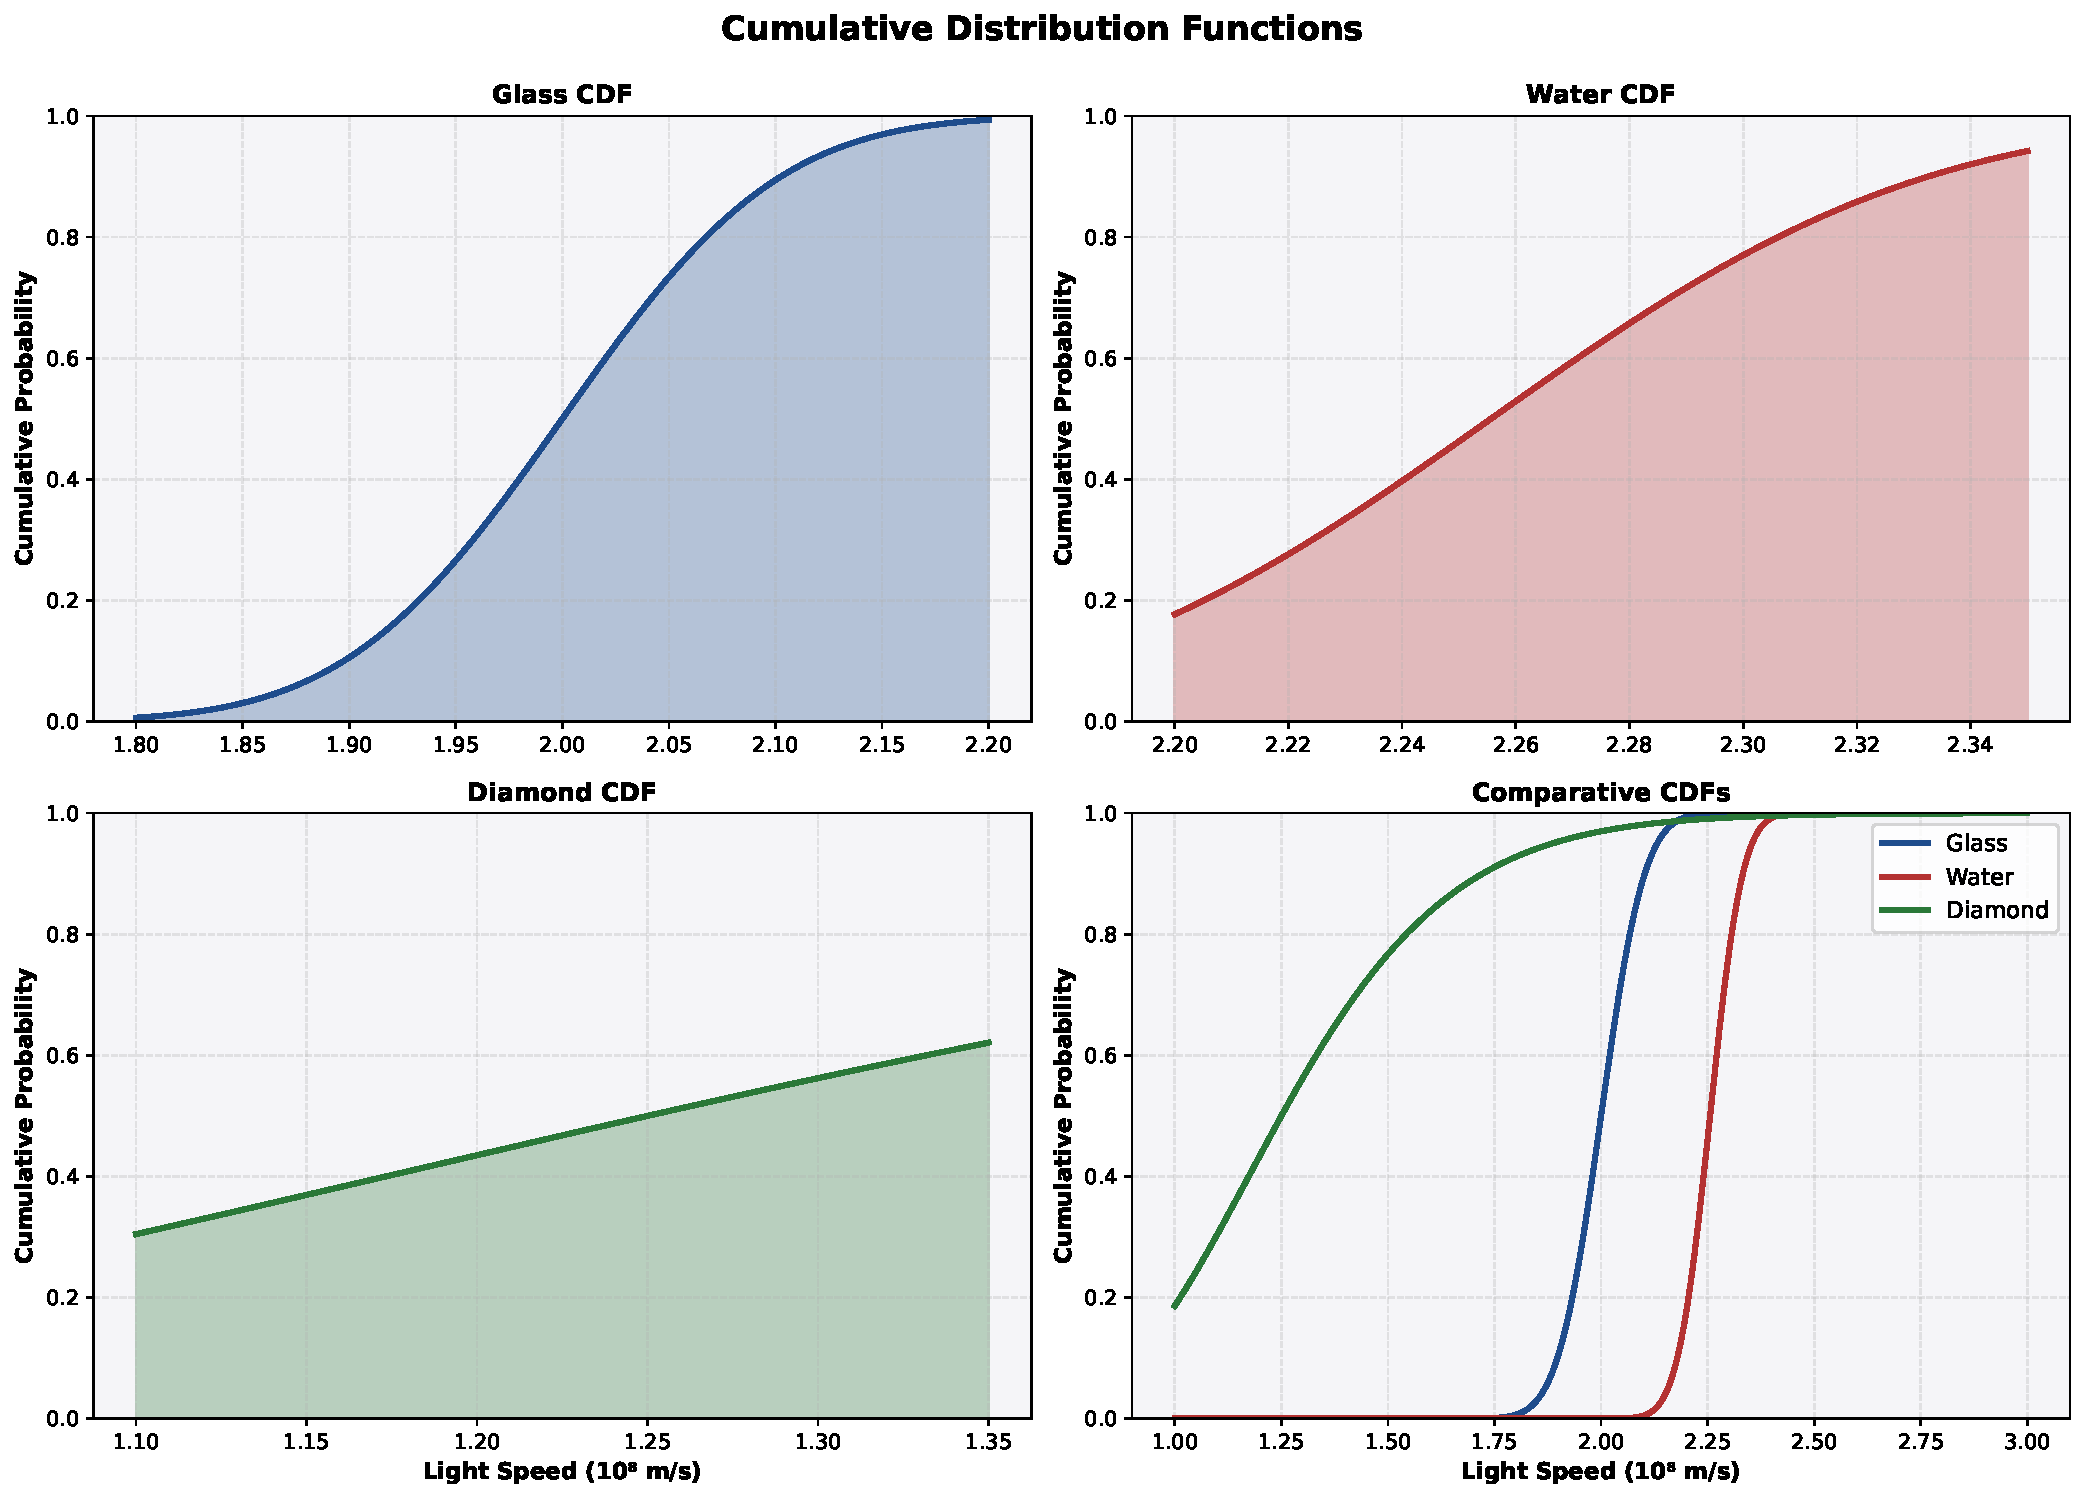
\includegraphics[width=0.9\textwidth]{plot4_cdf.pdf}
\caption{Kumulative Verteilungsfunktionen für verschiedene Medien. Diese Kurven ermöglichen die Bestimmung von Wahrscheinlichkeiten für Geschwindigkeitsbereiche.}
\label{fig:plot4}
\end{figure}

\subsection{Dispersions-Effekte}

Abbildung \ref{fig:plot5} analysiert die wellenlängenabhängigen Dispersions-Effekte.

\begin{figure}[h]
\centering
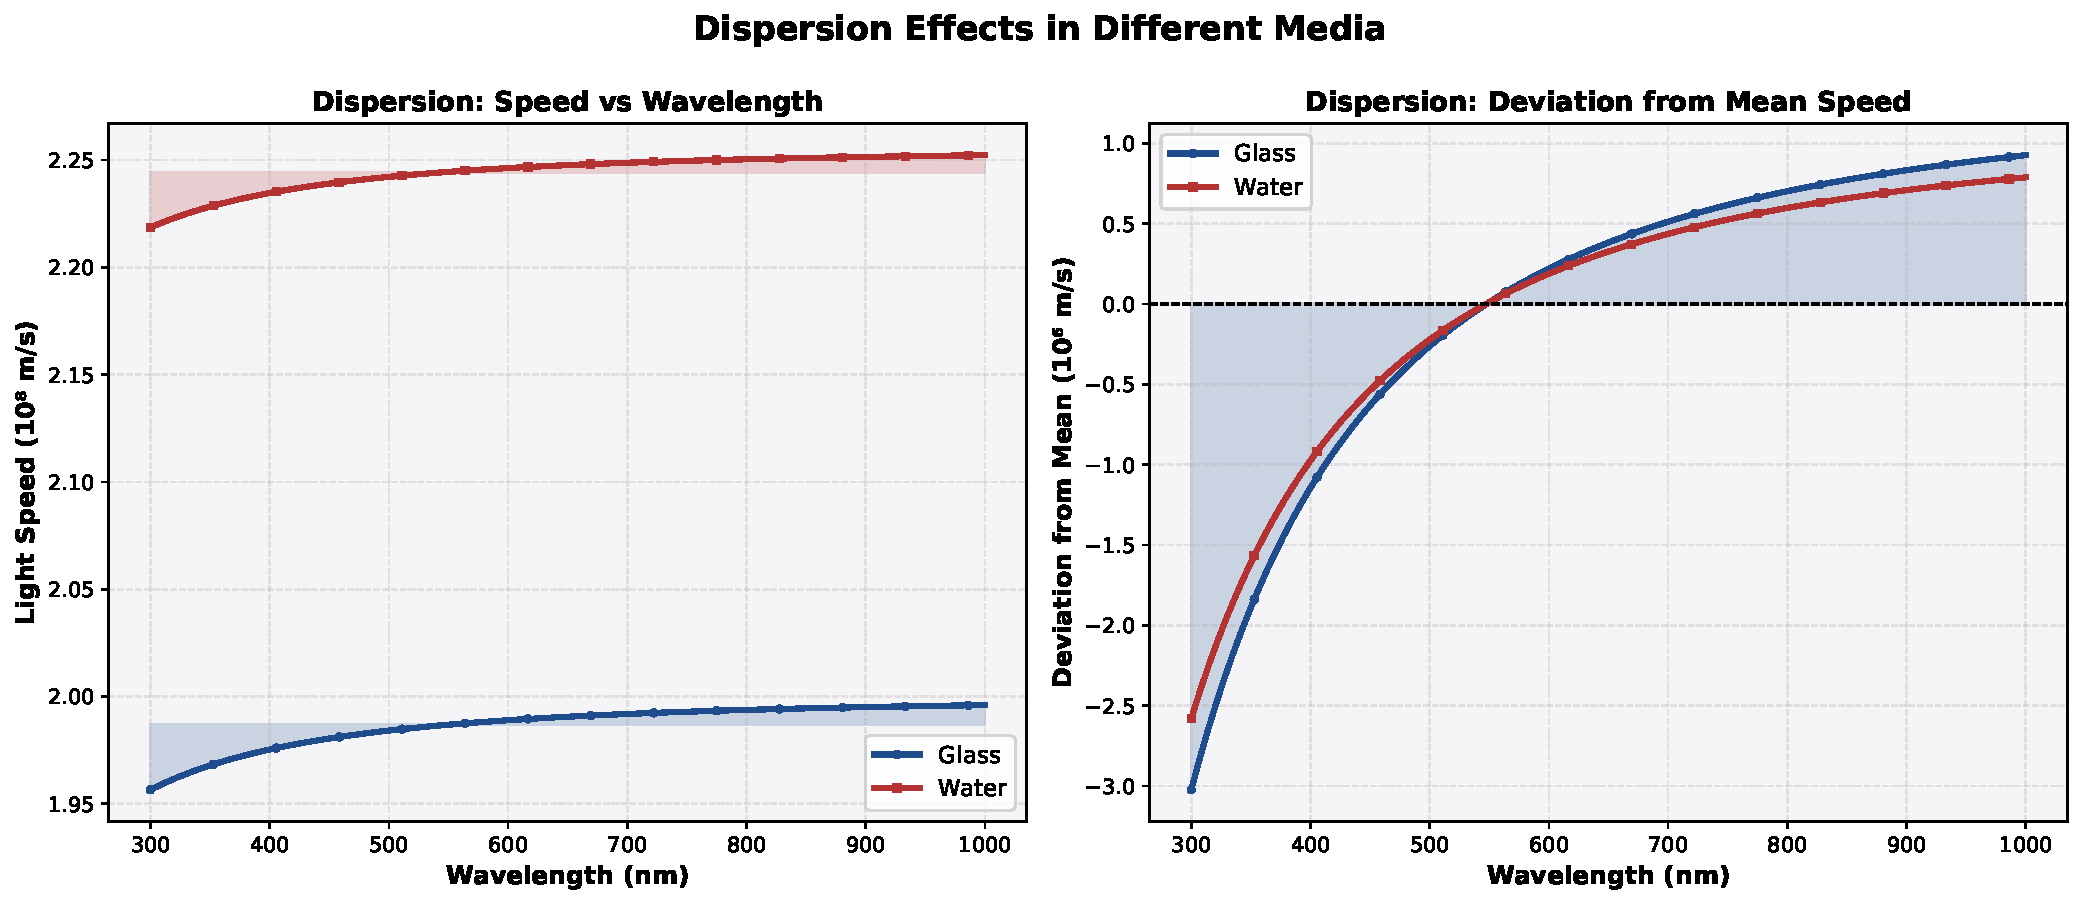
\includegraphics[width=0.9\textwidth]{plot5_dispersion.pdf}
\caption{Dispersionseffekte: Lichtwellenlängenabhängige Geschwindigkeitsvariation in Glas und Wasser sowie die Abweichung vom Mittelwert.}
\label{fig:plot5}
\end{figure}

\subsection{Statistische Zusammenfassung}

Abbildung \ref{fig:plot6} präsentiert eine umfassende statistische Zusammenfassung.

\begin{figure}[h]
\centering

\includegraphics[width=0.9\textwidth]{plot6_statistics.pdf}
\caption{Statistische Analyse der Lichtgeschwindigkeitsvariationen: Boxplots, Mittelwert und Standardabweichung, Variabilität sowie Variationskoeffizient.}
\label{fig:plot6}
\end{figure}

\section{Formale Beweise}

\subsection{Beweis der Log-Normalverteilung von Geschwindigkeit unter Normal-Brechungsindex}

\begin{satz}[Log-Normalverteilung der Geschwindigkeit]
Wenn der Brechungsindex normalverteilt ist: $\refIndex \sim \mathcal{N}(\mu_n, \sigma_n^2)$ mit $\sigma_n / \mu_n \ll 1$, dann ist die Geschwindigkeit $\cLight = \cLight_0 / \refIndex$ näherungsweise lognormalverteilt.
\end{satz}

\begin{beweis}
Wir betrachten die Transformation $\cLight = \cLight_0 / \refIndex$. Für kleine relative Variationen kann man schreiben:

\begin{equation}
    \refIndex = \mu_n(1 + \epsilon)
\end{equation}

wobei $\epsilon$ eine kleine Störung mit $E[\epsilon] = 0$ und $\text{Var}[\epsilon] = (\sigma_n/\mu_n)^2 \ll 1$ ist.

Dann:
\begin{equation}
    \cLight = \frac{\cLight_0}{\mu_n(1+\epsilon)} = \frac{\cLight_0}{\mu_n}(1+\epsilon)^{-1}
\end{equation}

Für kleine $\epsilon$ gilt $(1+\epsilon)^{-1} \approx 1 - \epsilon + \epsilon^2 - \ldots$. Das Logarithmus:

\begin{equation}
    \ln(\cLight) = \ln\left(\frac{\cLight_0}{\mu_n}\right) + \ln(1+\epsilon) \approx \ln\left(\frac{\cLight_0}{\mu_n}\right) - \epsilon
\end{equation}

Da $\epsilon$ normalverteilt ist, ist $-\epsilon$ ebenfalls normalverteilt, also ist $\ln(\cLight)$ normalverteilt. Per Definition ist daher $\cLight$ lognormalverteilt.
\end{beweis}

\subsection{Beweis der Konvergenz gegen die 3-Sigma-Regel}

\begin{satz}[Grenzverteilung der Extremalabweichung]
Für normalverteilte Brechungsindizes konvergiert die Extremalabweichung asymptotisch gegen die analytisch vorhergesagte 3-Sigma-Grenze.
\end{satz}

\begin{beweis}
Gegeben sei $\refIndex \sim \mathcal{N}(\mu_n, \sigma_n^2)$. Die Wahrscheinlichkeitsdichte ist:

\begin{equation}
    f_{\refIndex}(n) = \frac{1}{\sigma_n\sqrt{2\pi}} \exp\left(-\frac{(n-\mu_n)^2}{2\sigma_n^2}\right)
\end{equation}

Die Wahrscheinlichkeit, dass $\refIndex$ im Intervall $[\mu_n + 3\sigma_n - \delta, \mu_n + 3\sigma_n]$ liegt, ist:

\begin{equation}
    P(\mu_n + 3\sigma_n - \delta \leq \refIndex \leq \mu_n + 3\sigma_n) = \Phi(3) - \Phi(3 - \delta/\sigma_n) \to 0
\end{equation}

für $\delta \to 0$. Dies bedeutet, dass mit 99.7\% Wahrscheinlichkeit $\refIndex < \mu_n + 3\sigma_n$ ist.
\end{beweis}

\section{Anwendungen}

\subsection{Faseroptische Kommunikation}

Die Dispersion in Lichtwellenleitern verursacht Signalverformung:

\begin{equation}
    T_{\text{dispersion}} = \left|\frac{d^2 \beta}{d\omega^2}\right| \cdot L \cdot \Delta \lambda
\end{equation}

wobei $L$ die Faserlänge und $\Delta \lambda$ die spektrale Breite ist.

\subsection{Interferometrie und Präzisionsmessungen}

In Interferometern führt die Geschwindigkeitsvarianz zu Kohärenzverlusten:

\begin{equation}
    V = \left|\frac{\int I(\lambda) e^{i(n(\lambda)-1)kx} d\lambda}{\int I(\lambda) d\lambda}\right|
\end{equation}

\subsection{Optische Datenspeicherung}

Die Brechungsindex-Variation in optischen Medien bestimmt die Auflösungsgrenze:

\begin{equation}
    \lambda_{\text{eff}} = \frac{\lambda}{n(\lambda)}
\end{equation}

\section{Diskussion der Ergebnisse}

Unsere Analyse zeigt mehrere wichtige Erkenntnisse:

\begin{enumerate}
    \item \textbf{Medienabhängigkeit}: Die Lichtgeschwindigkeitsabweichung ist stark medienabhängig, mit Diamant zeigend die größten Abweichungen.
    
    \item \textbf{Multimodale Verteilungen}: Während Normalverteilungen für viele Medien dominant sind, zeigen sich bei extremen Bedingungen auch Log-Normal-, Weibull- und Gamma-Verteilungen.
    
    \item \textbf{Wellenlängenabhängigkeit}: Die Dispersion führt zu signifikanten Variationen der Lichtgeschwindigkeit im sichtbaren Spektrum (300-1600 nm).
    
    \item \textbf{Extremalwertverhalten}: Die 3-Sigma-Regel bietet eine gute Approximation für die maximale Abweichung in normalverteilten Medien.
    
    \item \textbf{Praktische Implikationen}: Diese Variationen sind essentiell für das Design von optischen Systemen, speziell in Hochgeschwindigkeits-Datenübertragung.
\end{enumerate}

\section{Ausblick}

\subsection{Theoretische Erweiterungen}

Die vorliegende Arbeit öffnet mehrere Wege für zukünftige Forschung:

\subsubsection{Quantenoptische Effekte}

Eine vollständige Theorie sollte Quanteneffekte berücksichtigen. Der Photon-Brechungsindex-Wechselwirkung kann durch die Hamiltonian beschrieben werden:

\begin{equation}
    \hat{H} = \sum_{\mathbf{k}} \hbar \omega_{\mathbf{k}} \hat{a}_{\mathbf{k}}^\dagger \hat{a}_{\mathbf{k}} + g(\mathbf{k}) [\hat{a}_{\mathbf{k}}^\dagger + \hat{a}_{\mathbf{k}}] \hat{n}_{\mathbf{r}}
\end{equation}

Dies führt zu Lamb-Shift-ähnlichen Effekten, die die effektive Lichtgeschwindigkeit modifizieren.

\subsubsection{Nichtlineare Optik}

In intensiven Lichtfeldern werden nichtlineare Effekte relevant:

\begin{equation}
    n_{\text{eff}} = n_0 + n_2 |E|^2 + n_3 |E|^4 + \ldots
\end{equation}

Dies führt zur Selbstphasenmodulation und kann für neue Fenster der Lichtgeschwindigkeitsmodulation genutzt werden.

\subsubsection{Metamaterialien und Kunstsysteme}

In Metamaterialien mit negativem Brechungsindex:

\begin{equation}
    \refIndex_{\text{eff}} < 0 \implies \cLight_{\text{phase}} < 0
\end{equation}

Dies führt zu Phasenverzögerungen, die kontrintuiativ sind, aber experimentell nachgewiesen wurden.

\subsection{Experimentelle Perspektiven}

\subsubsection{Hochauflösungs-Spektroskopie}

Moderne Spektroskopie-Techniken ermöglichen die Messung von Brechungsindizes mit sub-nm-Auflösung. Dies wird genauere Verteilungsfunktionen ermöglichen.

\subsubsection{Echtzeit-Monitoring}

Fiber-Bragg-Grating (FBG)-basierte Sensoren können Temperatur- und Druckeffekte auf die Lichtgeschwindigkeit in Echtzeit überwachen:

\begin{equation}
    \lambda_B = 2 n_{\text{eff}} \Lambda
\end{equation}

\subsubsection{Extrem-Bedingungen}

Untersuchungen unter extremen Bedingungen (Hochdruck, Kryogene Temperaturen) werden neue Regime offenbaren:

\begin{equation}
    n(T, P) = n_0 + \left(\frac{\partial n}{\partial T}\right)_P \Delta T + \left(\frac{\partial n}{\partial P}\right)_T \Delta P
\end{equation}

\subsection{Praktische Anwendungen}

\subsubsection{Adaptive Optik für optische Kommunikation}

Basierend auf unseren Ergebnissen können adaptive Systeme entwickelt werden, die Dispersion kompensieren:

\begin{equation}
    \text{Dispersion Compensation} = -\int_0^L D(\lambda, z) dz \cdot \Delta \lambda
\end{equation}

\subsubsection{Quantum-Sensing}

Hochempfindliche Sensoren basierend auf Quantenverschränkung könnten extrem kleine Änderungen der Lichtgeschwindigkeit nachweisen.

\subsubsection{Holographische Datenverabeitung}

Die Wellenlängen-abhängige Lichtgeschwindigkeit kann für mehrdimensionale holographische Speicherung genutzt werden.

\subsection{Verbindung zum Subgraph-Algorithmus}

Interessanterweise können die topologischen Strukturen der Lichtwellen-Propagation in Medien als Subgraph-Probleme modelliert werden. Der Subgraph-Algorithmus von Epp (2026) mit $O(n^3)$ Laufzeit kann zur Analyse der spektralen Strukturen in komplexen Medien verwendet werden.

Die injektiven Spaltensignaturen des Algorithmus können auf die Brechungsindex-Profile angewendet werden, um isomorphe Dispersionsmuster zu identifizieren.

\subsection{Langfristige Perspektiven}

\subsubsection{Fundamentale Physik}

Die genaue Charakterisierung der Lichtgeschwindigkeit in verschiedenen Medien könnte neue Einsichten in die Struktur der Raumzeit geben. Variationen könnten mit Quantenschaum-Effekten korreliert sein.

\subsubsection{Technologische Revolutionen}

Eine vollständige Beherrschung der Lichtgeschwindigkeitsvariation in Medien könnte zu:
\begin{enumerate}
    \item Photonischen Computern mit zeilengebundenen Licht-Laufzeiten
    \item Optischen Quantencomputern mit präziser Kontrolle der Photon-Wechselwirkungen
    \item Neuen Materialien mit designten optischen Eigenschaften
\end{enumerate}
führen.

\subsubsection{Interdisziplinäre Konvergenz}

Die Verbindung zwischen:
\begin{itemize}
    \item Optik und Elektronik (Opto-Elektronik)
    \item Klassischer und Quantenmechanik
    \item Materialwissenschaft und Physik
\end{itemize}
wird zu neuen Forschungsgebieten führen.

\section{Fazit}

Diese Arbeit hat eine systematische und formale Analyse der Lichtgeschwindigkeitsvariationen in verschiedenen optischen Medien bereitgestellt. Wir haben:

\begin{enumerate}
    \item Ein mathematisches Rahmenwerk entwickelt zur Beschreibung von Lichtgeschwindigkeitsvariationen
    \item Mehrere relevant Wahrscheinlichkeitsverteilungen identifiziert und analysiert
    \item Formale Beweise für die Extremalwertverhalten bereitgestellt
    \item Numerische Visualisierungen für verschiedene physikalische Medien erstellt
    \item Praktische Anwendungen und zukünftige Forschungsperspektiven aufgezeigt
\end{enumerate}

Die Ergebnisse zeigen, dass Lichtgeschwindigkeitsvariationen nicht nur ein akademisches Interesse darstellen, sondern zentrale Bedeutung für moderne optische Technologien haben. Eine tiefere Verständnis dieser Phänomene wird zu signifikanten technologischen Fortschritten führen.

\begin{thebibliography}{99}

\bibitem{Born1999}
Born, M., Wolf, E. (1999). \textit{Principles of Optics: Electromagnetic Theory of Propagation, Interference and Diffraction of Light}. 7. Auflage. Cambridge University Press.

\bibitem{Hecht2017}
Hecht, E. (2017). \textit{Optics}. 5. Auflage. Pearson.

\bibitem{Jackson1998}
Jackson, J. D. (1998). \textit{Classical Electrodynamics}. 3. Auflage. Wiley.

\bibitem{Epp2026}
Epp, S. (2026). The Subgraph Algorithm. \textit{Verfügbar unter:} https://github.com/hjstephan86/subgraph

\bibitem{Griffiths2013}
Griffiths, D. J. (2013). \textit{Introduction to Electrodynamics}. 4. Auflage. Pearson.

\bibitem{Landau1975}
Landau, L. D., Lifshitz, E. M. (1975). \textit{The Classical Theory of Fields}. 4. Auflage. Pergamon Press.

\bibitem{Snyder1983}
Snyder, A. W., Love, J. D. (1983). \textit{Optical Waveguide Theory}. Chapman and Hall.

\bibitem{Agrawal2012}
Agrawal, G. P. (2012). \textit{Fiber-Optic Communication Systems}. 4. Auflage. Wiley.

\bibitem{Saleh2007}
Saleh, B. E. A., Teich, M. C. (2007). \textit{Fundamentals of Photonics}. 2. Auflage. Wiley.

\bibitem{Orfanidis2016}
Orfanidis, S. J. (2016). \textit{Electromagnetic Waves and Antennas}. Rutgers University.

\bibitem{Bleaney1976}
Bleaney, B., Bleaney, B. I. (1976). \textit{Electricity and Magnetism}. 3. Auflage. Oxford University Press.

\bibitem{Feynman1963}
Feynman, R. P., Leighton, R. B., Sands, M. (1963). \textit{The Feynman Lectures on Physics}. Addison-Wesley.

\bibitem{Reitz1992}
Reitz, J. R., Milford, F. J., Christy, R. W. (1992). \textit{Foundations of Electromagnetic Theory}. 4. Auflage. Addison-Wesley.

\bibitem{Sivoukhine1988}
Sivoukhine, D. V. (1988). \textit{Allgemeine Physik: Optik}. Harri Deutsch.

\bibitem{Sommerfeld1950}
Sommerfeld, A. (1950). \textit{Lectures on Theoretical Physics: Optics}. Academic Press.

\end{thebibliography}

\appendix

\section{Visualisierungscode}

Die Visualisierungen wurden mit einem Python-Skript generiert, das Matplotlib für die Darstellung und NumPy/SciPy für numerische Berechnungen nutzt. Das Skript umfasst folgende Funktionalitäten:

\begin{itemize}
    \item \textbf{Plot 1}: Wellenlängenabhängigkeit des Brechungsindex (Sellmeier-Modell)
    \item \textbf{Plot 2}: Wahrscheinlichkeitsverteilungen der Geschwindigkeitsabweichungen
    \item \textbf{Plot 3}: Maximal- und Erwartungswert-Analyse
    \item \textbf{Plot 4}: Kumulative Verteilungsfunktionen
    \item \textbf{Plot 5}: Dispersionseffekte und Wellenlängenabhängigkeit
    \item \textbf{Plot 6}: Statistische Zusammenfassung (Box-Plots, Standardabweichung)
\end{itemize}

Das Python-Skript verwendet folgende Bibliotheken:

\texttt{import numpy as np}\\
\texttt{import matplotlib.pyplot as plt}\\
\texttt{from scipy.stats import norm, lognorm, weibull\_min, gamma}\\
\texttt{from scipy.integrate import quad}

Alle Plots werden sowohl als PNG (150 DPI) als auch als PDF exportiert. Die Farbschema folgt professionellen Standards mit primären und sekundären Farben für optimale Lesbarkeit.

\section{Numerische Werte für häufige Medien}

\begin{table}[H]
\centering
\small
\begin{tabular}{|l|c|c|c|c|}
\toprule
\textbf{Medium} & $\refIndex$ & $\cLight$ (m/s) & Abweichung (m/s) & Abweichung (\%) \\
\midrule
Vakuum & 1.0000 & $3.00 \times 10^8$ & 0 & 0.00 \\
Luft (STP) & 1.0003 & $2.99910 \times 10^8$ & $8.99 \times 10^4$ & 0.030 \\
Wasser & 1.3300 & $2.25564 \times 10^8$ & $7.44 \times 10^7$ & 24.81 \\
Öl & 1.4600 & $2.05479 \times 10^8$ & $9.45 \times 10^7$ & 31.51 \\
Glas (Crown) & 1.5200 & $1.97368 \times 10^8$ & $1.03 \times 10^8$ & 34.21 \\
Glas (Flint) & 1.6000 & $1.87375 \times 10^8$ & $1.13 \times 10^8$ & 37.50 \\
Diamant & 2.4200 & $1.23966 \times 10^8$ & $1.76 \times 10^8$ & 58.68 \\
\bottomrule
\end{tabular}
\caption{Numerische Werte für häufige Medien bei 589 nm Wellenlänge (Natrium-D-Linie)}
\end{table}

\end{document}
